%======================================================================
\chapter{Implementation}
\label{ch: Chapter5}
%======================================================================

%======================================================================
\section{Experimental Setup}
%----------------------------------------------------------------------
\subsection{USB}
%----------------------------------------------------------------------


%----------------------------------------------------------------------
\subsection{Raspberry Pi}
%----------------------------------------------------------------------
The communication protocol utilized by the Q-Flex2 embedded panel is SPI.  
\begin{figure}[!htbp]
    \centering
    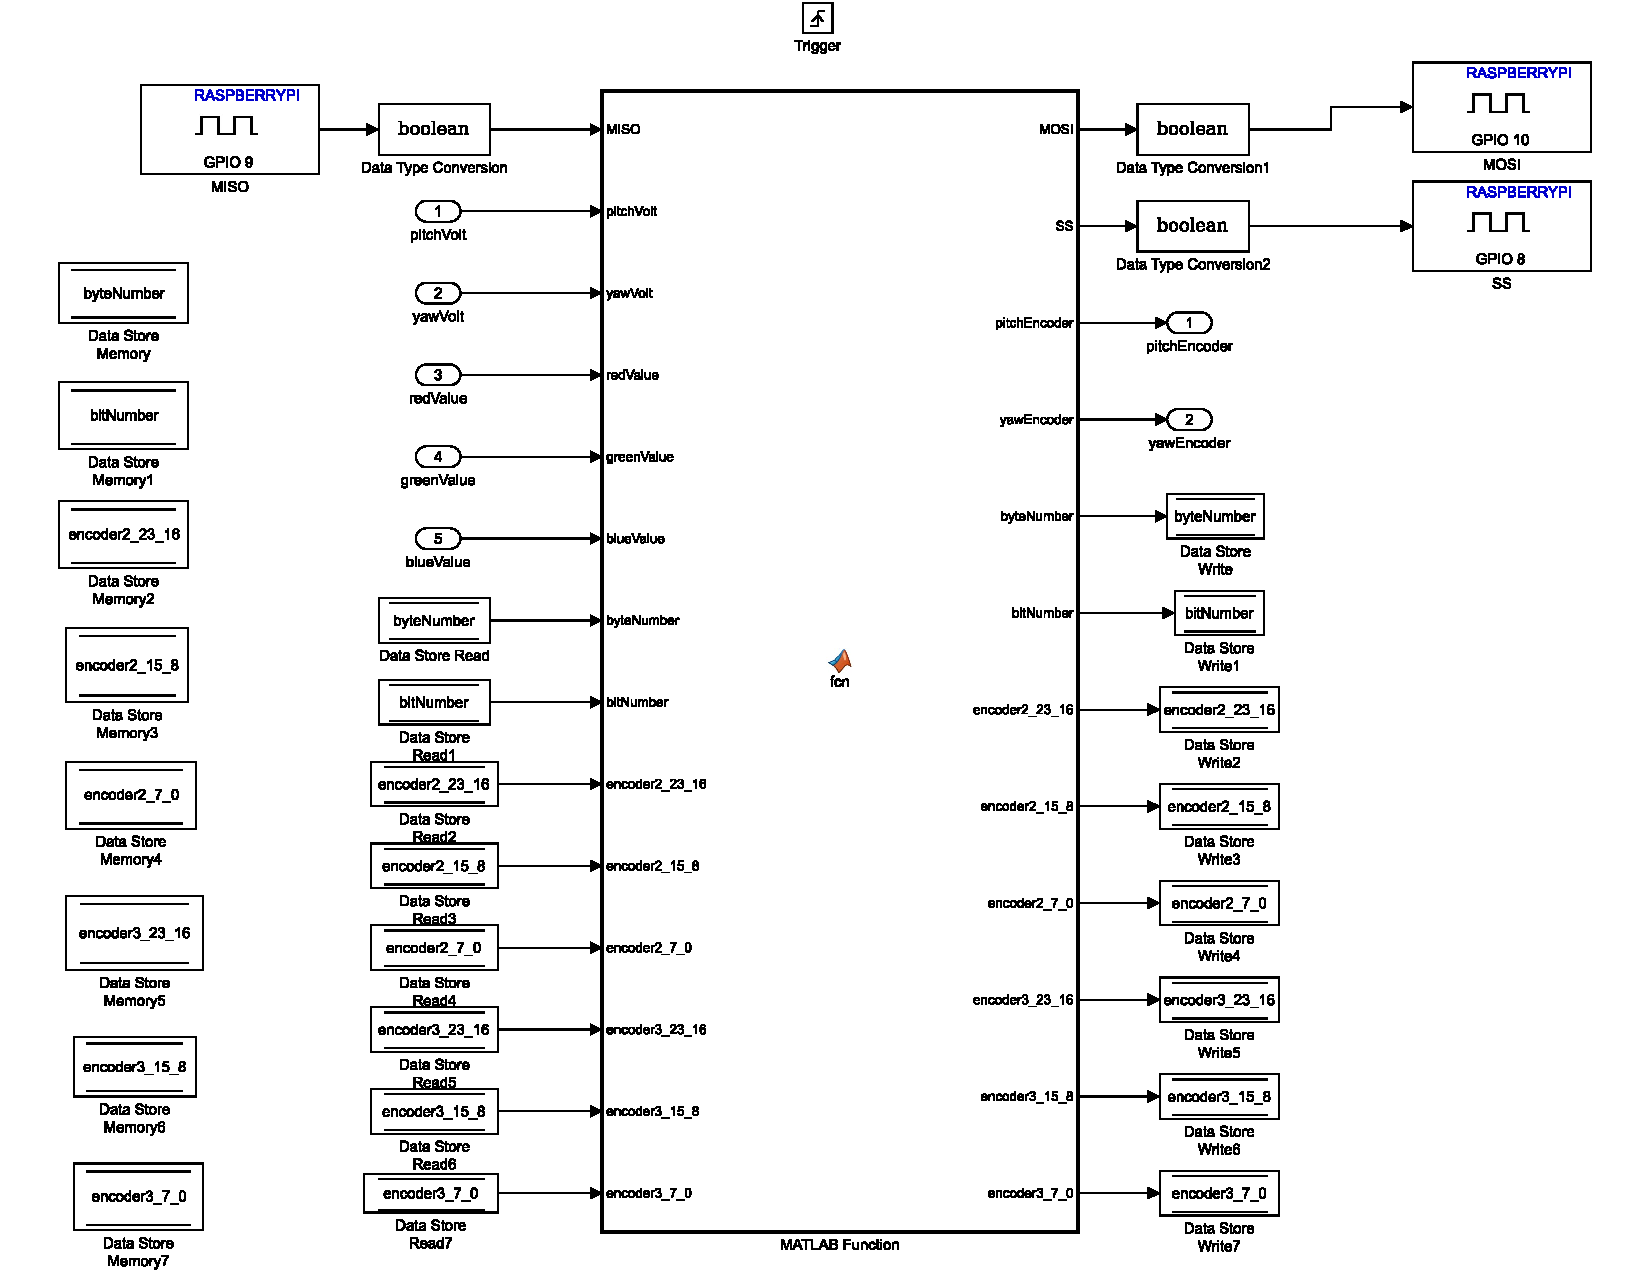
\includegraphics[width=.46\textwidth,keepaspectratio=true]{figs/img/SPI_COM.pdf}
    \label{fig:SPI_COM}
    \caption{Block diagram of SPI communication protocol used for communication between the Raspberry Pi and Quanser Aero.}
\end{figure}


%----------------------------------------------------------------------
\subsection{Android}
%----------------------------------------------------------------------
\begin{figure}[!htbp]
    \centering
    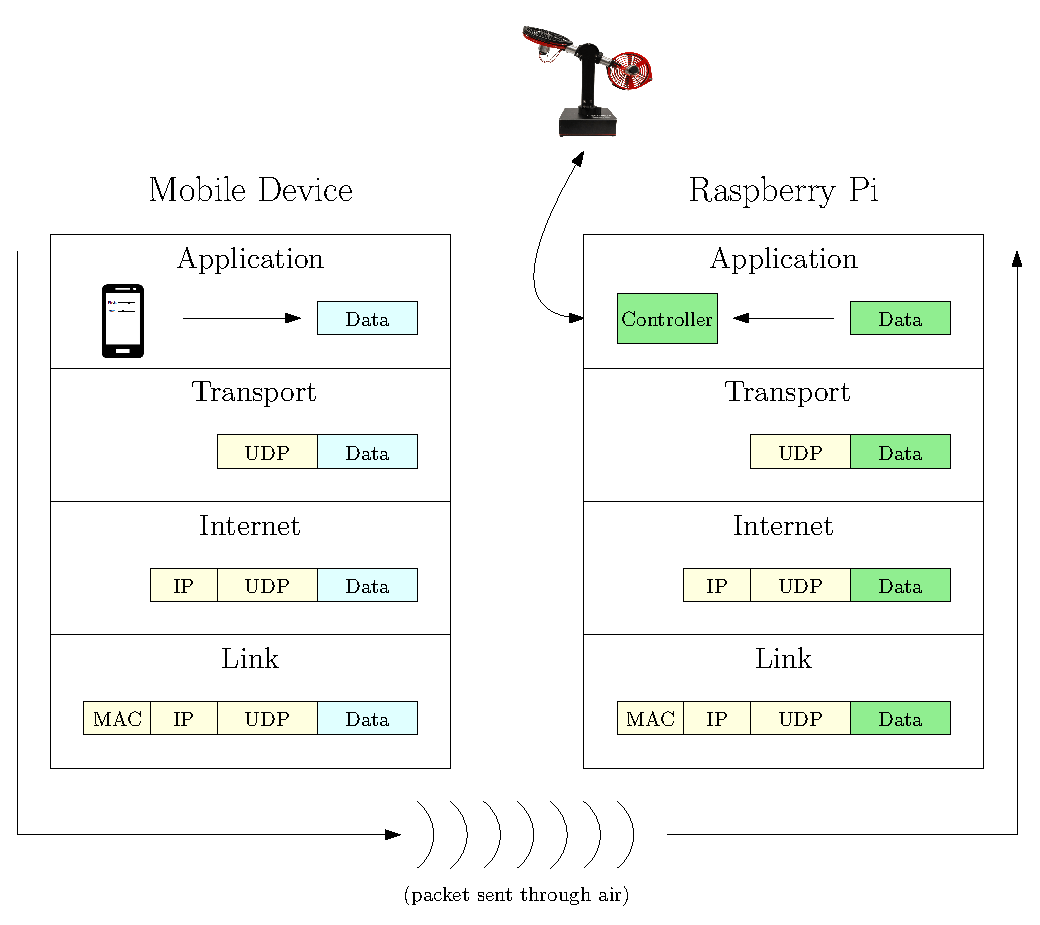
\includegraphics[width=.46\textwidth,keepaspectratio=true]{figs/ipe/TCPModel.eps}
    \label{fig:TCPModel}
    \caption{Illustration of the TCP model which describes how packets are sent and recieved from mobile devices to the Quanser Aero.}
\end{figure}

\begin{figure}[!htbp]
    \centering
    \includegraphics[width=.5\textwidth,keepaspectratio=true]{figs/ipe/Setup.eps}
    \label{fig:Setup}
    \caption{Experiment setup for controlling the Quanser Aeros via a mobile device.}
\end{figure}

%======================================================================
\section{USB}
%----------------------------------------------------------------------
\subsection{LQR}
%----------------------------------------------------------------------
\begin{figure}[!htbp]
    \centering
    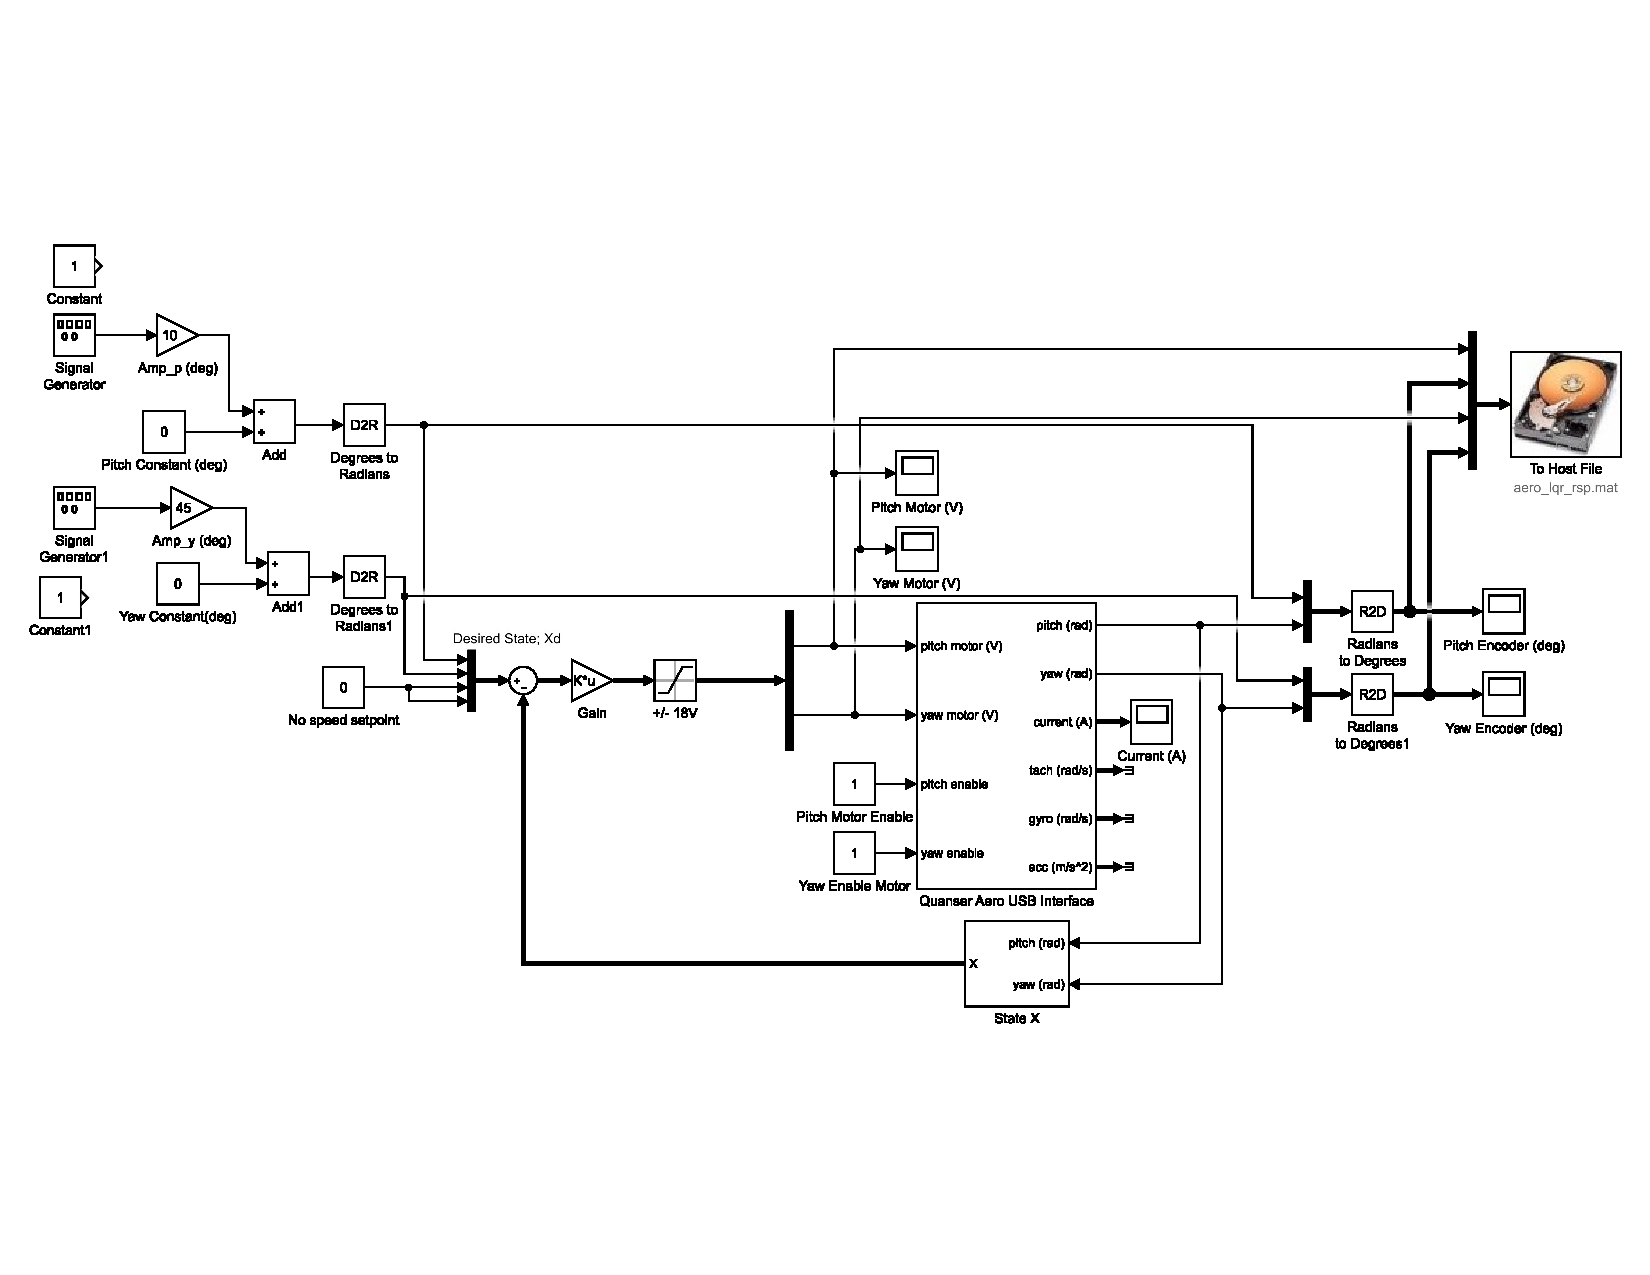
\includegraphics[width=.8\textwidth,keepaspectratio=true]{figs/img/LQR_USB}
    \label{fig:LQR_P_USB_Block_Diagram}
    \caption{Block Diagram for LQR P type controller with a USB connection.}
\end{figure}
\todo[inline]{Insert LQR PI Block Diagram}
%\begin{figure}[!htbp]
%    \centering
%    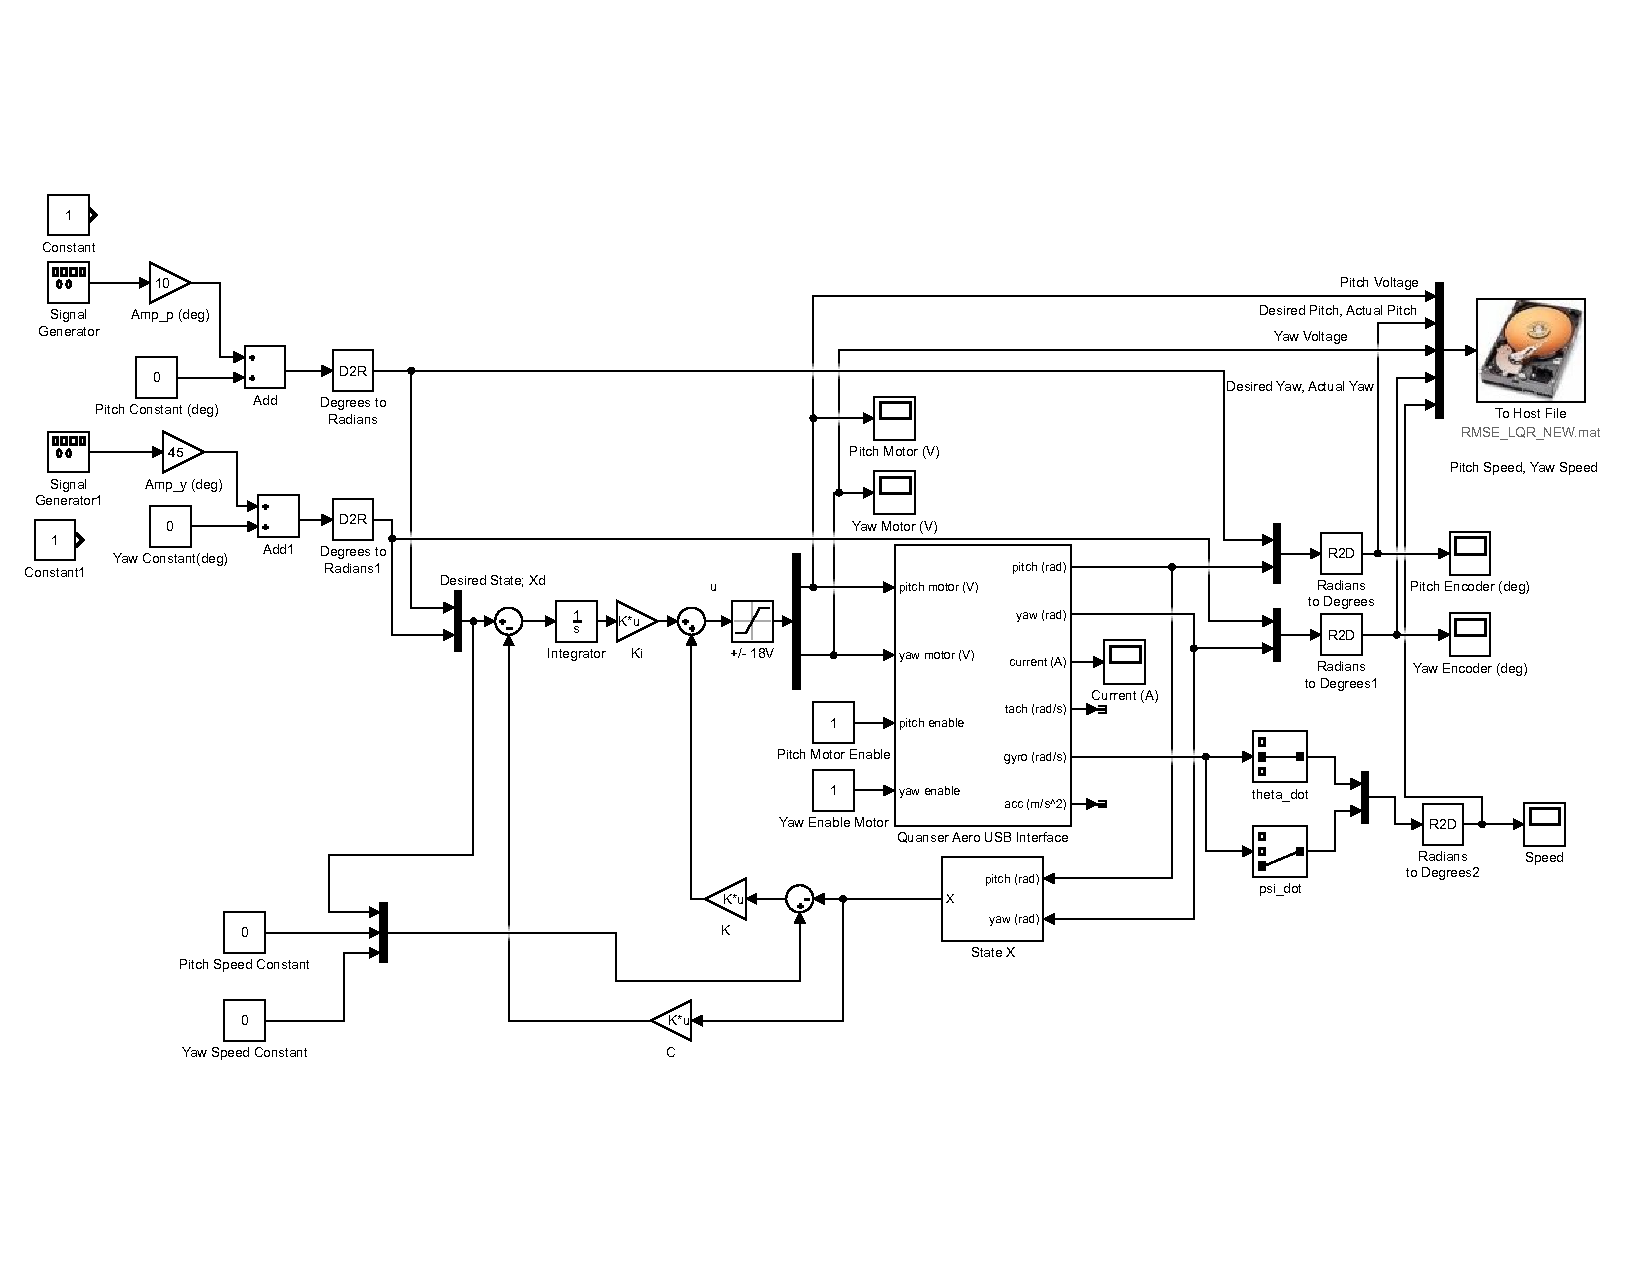
\includegraphics[width=.8\textwidth,keepaspectratio=true]{figs/img/LQR_PI_USB}
%    \label{fig:LQR_PI_USB_Block_Diagram}
%    \caption{Block Diagram for LQR PI type controller with a USB connection.}
%\end{figure}
\begin{figure}[!htbp]
    \centering
    \subfigure[][]{
    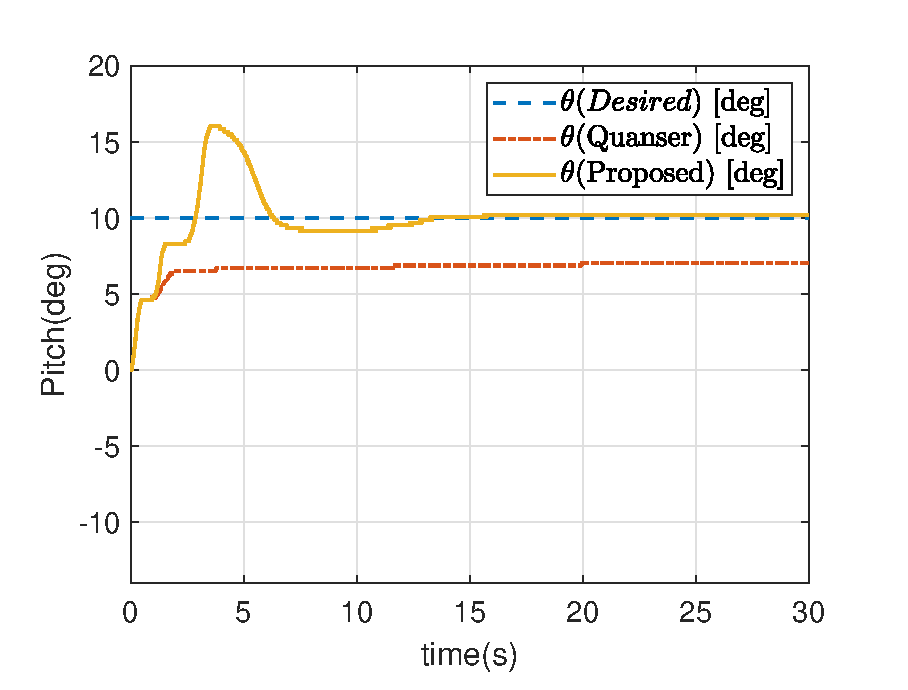
\includegraphics[width=.46\textwidth,keepaspectratio=true]{figs/matlab/LQR_PIvLQR_P_USB/step/Pitch_LQR_RMSE.eps}
    \label{fig:Pitch_LQR_RMSE_Step}
    }
    \subfigure[][]{
    \includegraphics[width=.46\textwidth,keepaspectratio=true]{figs/matlab/LQR_PIvLQR_P_USB/step/Yaw_LQR_RMSE.eps}
    \label{fig:Yaw_LQR_RMSE_Step}
    }    
    \subfigure[][]{
    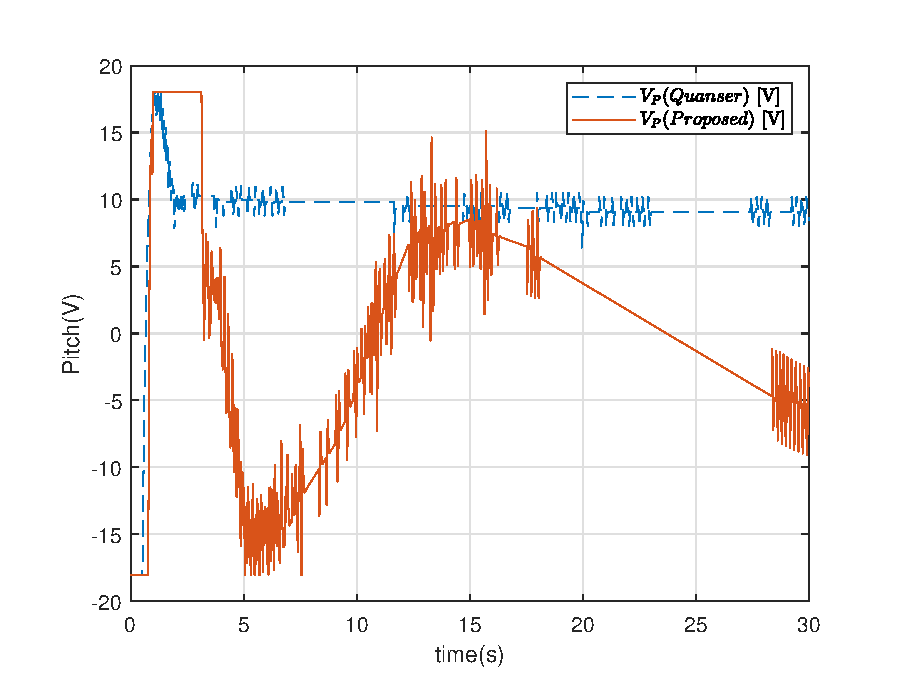
\includegraphics[width=.46\textwidth,keepaspectratio=true]{figs/matlab/LQR_PIvLQR_P_USB/step/PitchVoltage_LQR_RMSE.eps}
    \label{fig:PitchVoltage_LQR_RMSE_Step}
    }    
    \subfigure[][]{
    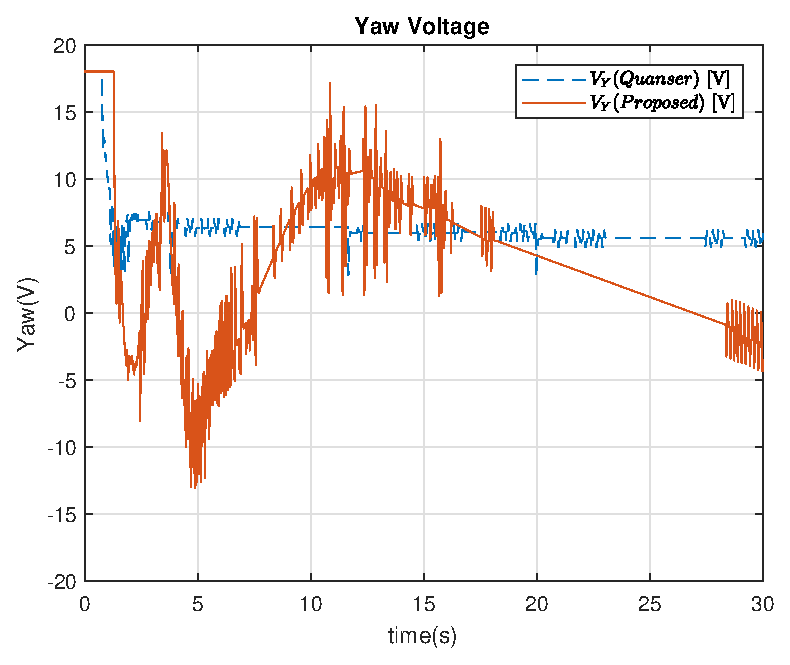
\includegraphics[width=.46\textwidth,keepaspectratio=true]{figs/matlab/LQR_PIvLQR_P_USB/step/YawVoltage_LQR_RMSE.eps}
    \label{fig:YawVoltage_LQR_RMSE_Step}
    }
    \subfigure[][]{
    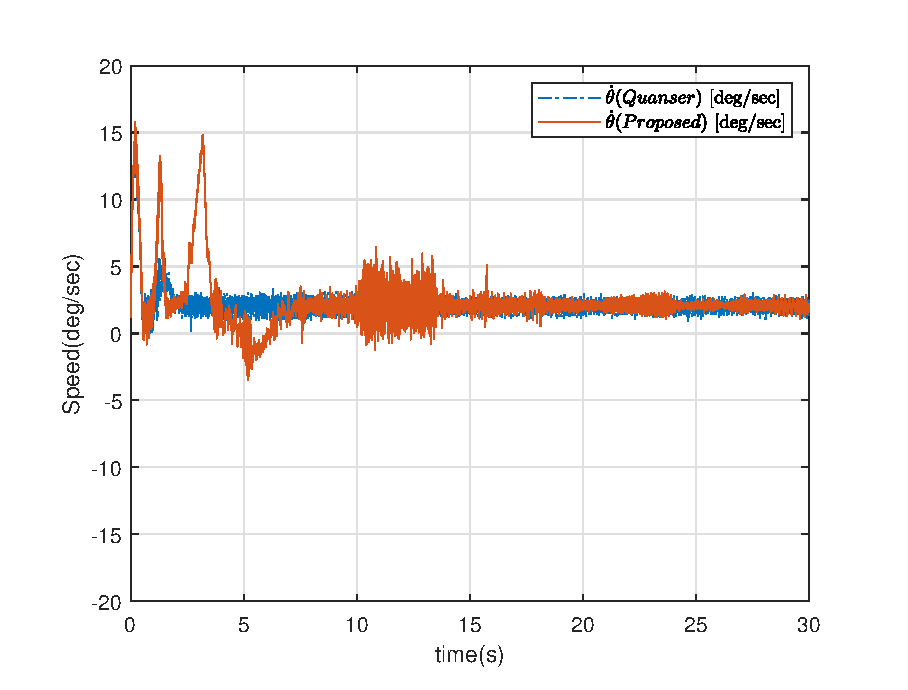
\includegraphics[width=.46\textwidth,keepaspectratio=true]{figs/matlab/LQR_PIvLQR_P_USB/step/PitchSpeed_LQR_RMSE.eps}
    \label{fig:PitchSpeed_LQR_RMSE_Step}
    }
    \subfigure[][]{
    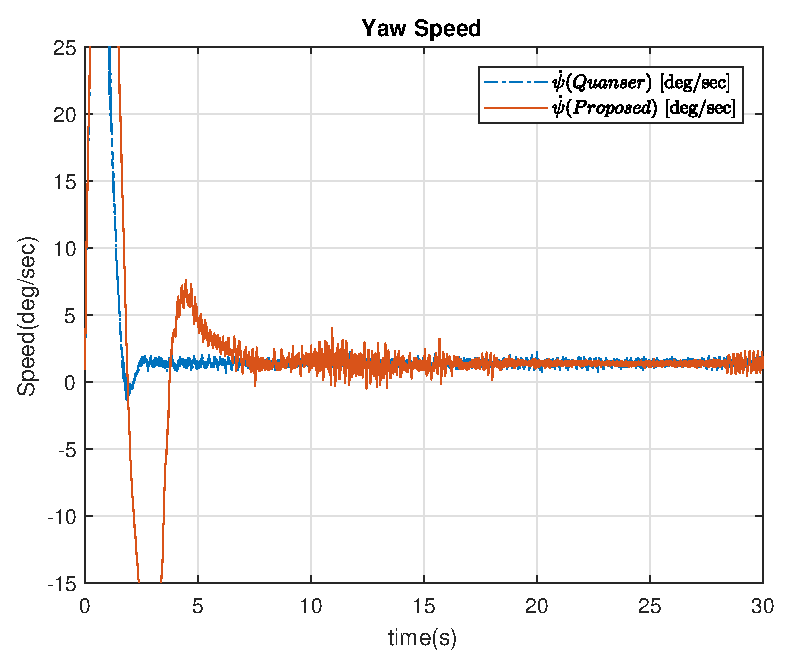
\includegraphics[width=.46\textwidth,keepaspectratio=true]{figs/matlab/LQR_PIvLQR_P_USB/step/YawSpeed_LQR_RMSE.eps}
    \label{fig:PitchSpeed_LQR_RMSE_Step}
    }
    \caption{USB implementation for proportional controller and proportional-integral controller calculated by LQR with a step input.}
\end{figure}

\begin{figure}[!htbp]
    \centering
    \subfigure[][]{
    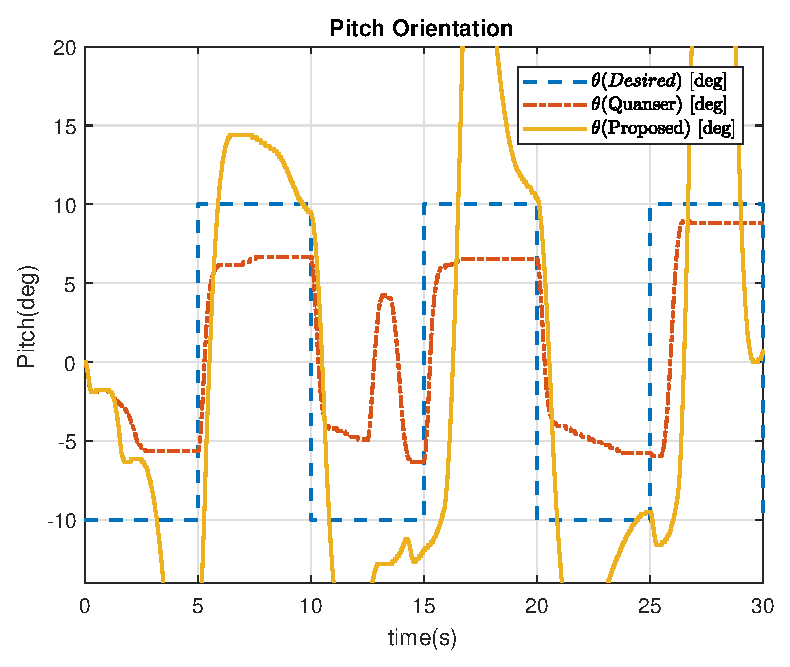
\includegraphics[width=.46\textwidth,keepaspectratio=true]{figs/matlab/LQR_PIvLQR_P_USB/square/Pitch_LQR_RMSE.eps}
    \label{fig:Pitch_LQR_RMSE_Square}
    }
    \subfigure[][]{
    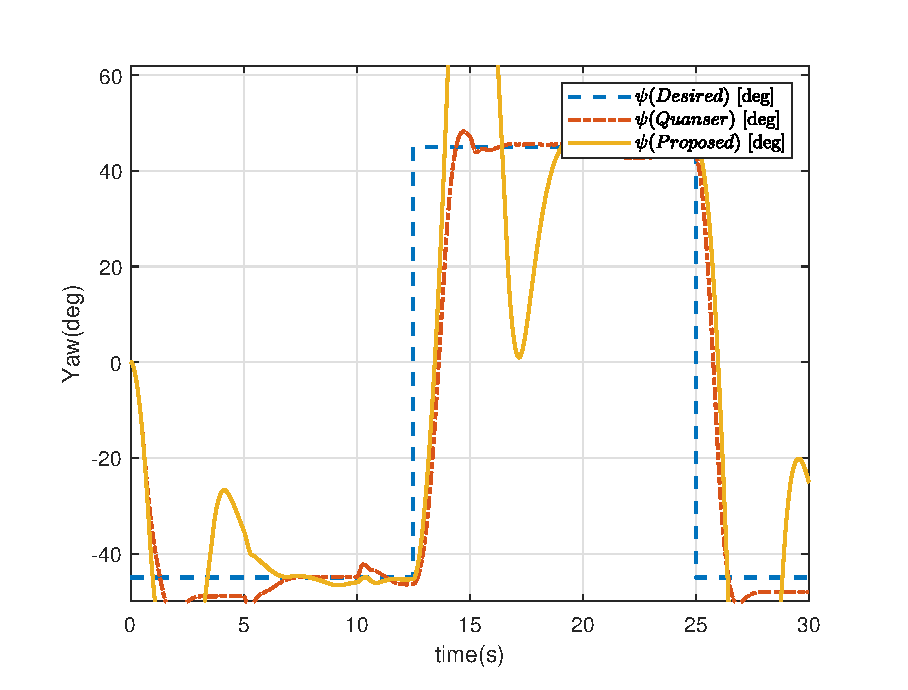
\includegraphics[width=.46\textwidth,keepaspectratio=true]{figs/matlab/LQR_PIvLQR_P_USB/square/Yaw_LQR_RMSE.eps}
    \label{fig:Yaw_LQR_RMSE_Square}
    }    
    \subfigure[][]{
    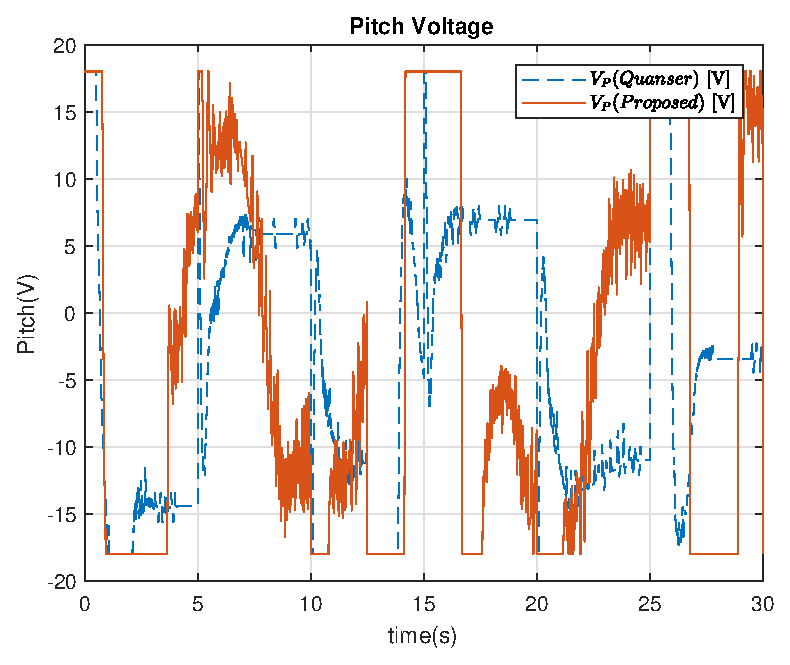
\includegraphics[width=.46\textwidth,keepaspectratio=true]{figs/matlab/LQR_PIvLQR_P_USB/square/PitchVoltage_LQR_RMSE.eps}
    \label{fig:PitchVoltage_LQR_RMSE_Square}
    }    
    \subfigure[][]{
    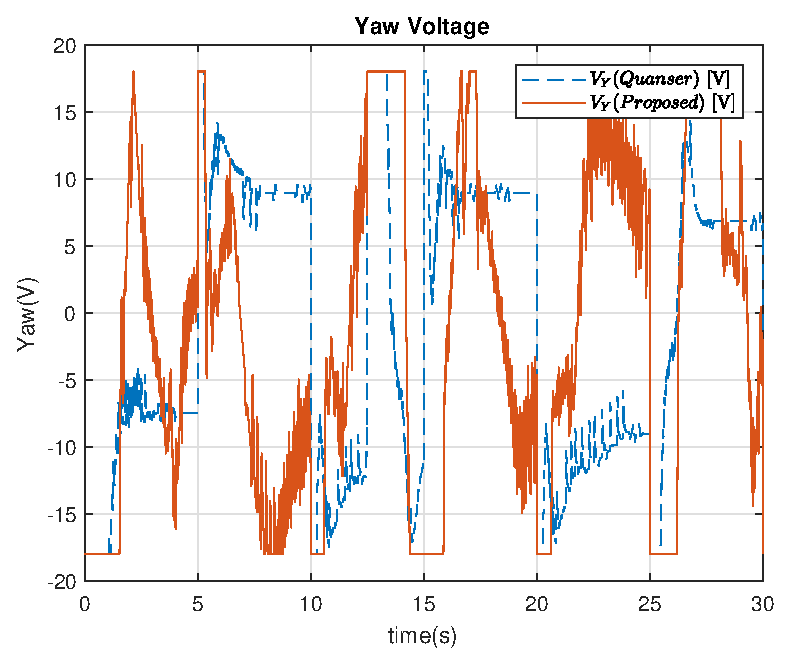
\includegraphics[width=.46\textwidth,keepaspectratio=true]{figs/matlab/LQR_PIvLQR_P_USB/square/YawVoltage_LQR_RMSE.eps}
    \label{fig:YawVoltage_LQR_RMSE_Square}
    }
    \subfigure[][]{
    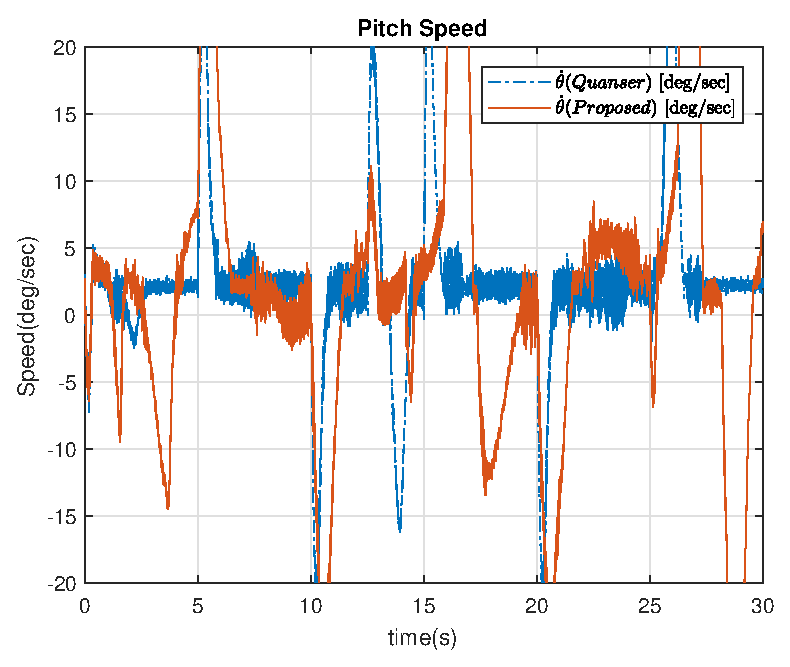
\includegraphics[width=.46\textwidth,keepaspectratio=true]{figs/matlab/LQR_PIvLQR_P_USB/square/PitchSpeed_LQR_RMSE.eps}
    \label{fig:PitchSpeed_LQR_RMSE_Square}
    }
    \subfigure[][]{
    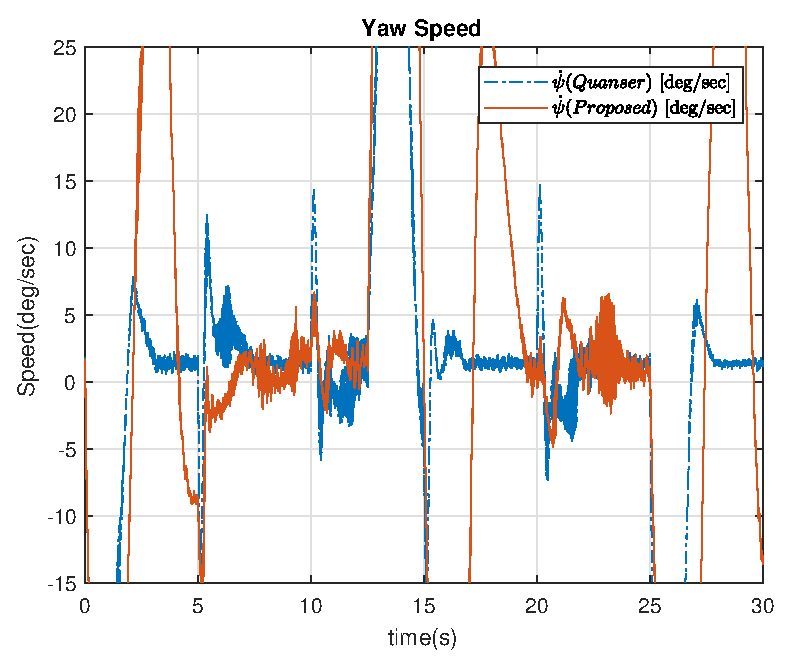
\includegraphics[width=.46\textwidth,keepaspectratio=true]{figs/matlab/LQR_PIvLQR_P_USB/square/YawSpeed_LQR_RMSE.eps}
    \label{fig:PitchSpeed_LQR_RMSE_Square}
    }
    \caption{USB implementation for proportional controller and proportional-integral controller calculated by LQR with a square wave input.}
\end{figure}

\begin{figure}[!htbp]
    \centering
    \subfigure[][]{
    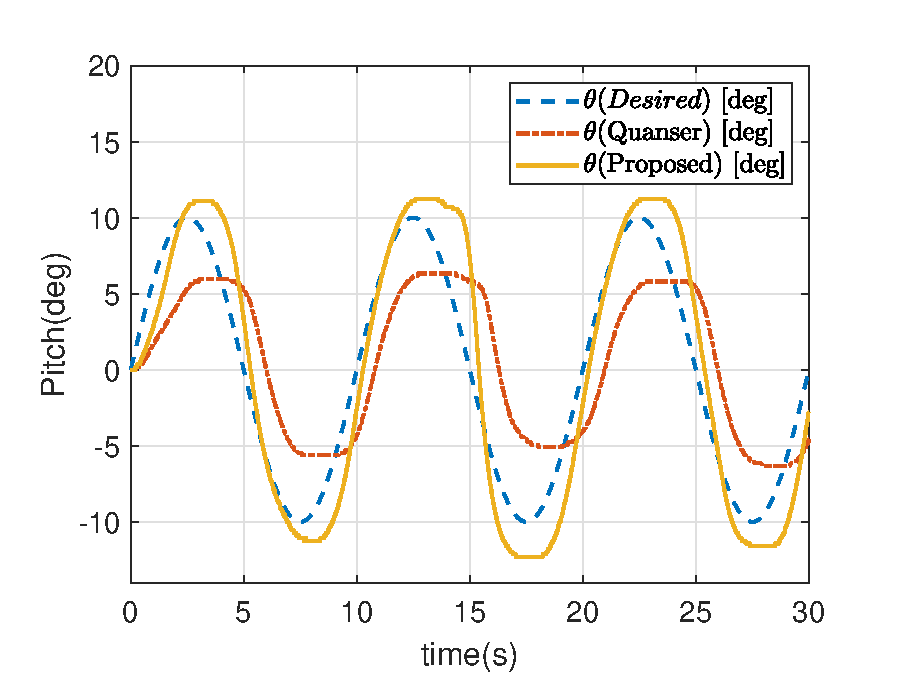
\includegraphics[width=.46\textwidth,keepaspectratio=true]{figs/matlab/LQR_PIvLQR_P_USB/sine/Pitch_LQR_RMSE.eps}
    \label{fig:Pitch_LQR_RMSE_Sine}
    }
    \subfigure[][]{
    \includegraphics[width=.46\textwidth,keepaspectratio=true]{figs/matlab/LQR_PIvLQR_P_USB/sine/Yaw_LQR_RMSE.eps}
    \label{fig:Yaw_LQR_RMSE_Sine}
    }    
    \subfigure[][]{
    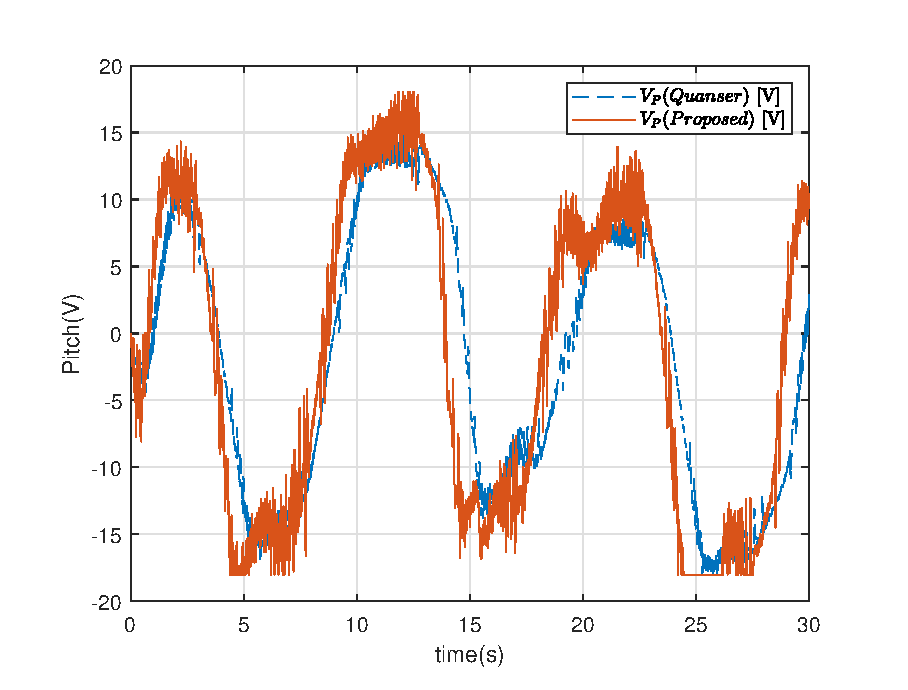
\includegraphics[width=.46\textwidth,keepaspectratio=true]{figs/matlab/LQR_PIvLQR_P_USB/sine/PitchVoltage_LQR_RMSE.eps}
    \label{fig:PitchVoltage_LQR_RMSE_Sine}
    }    
    \subfigure[][]{
    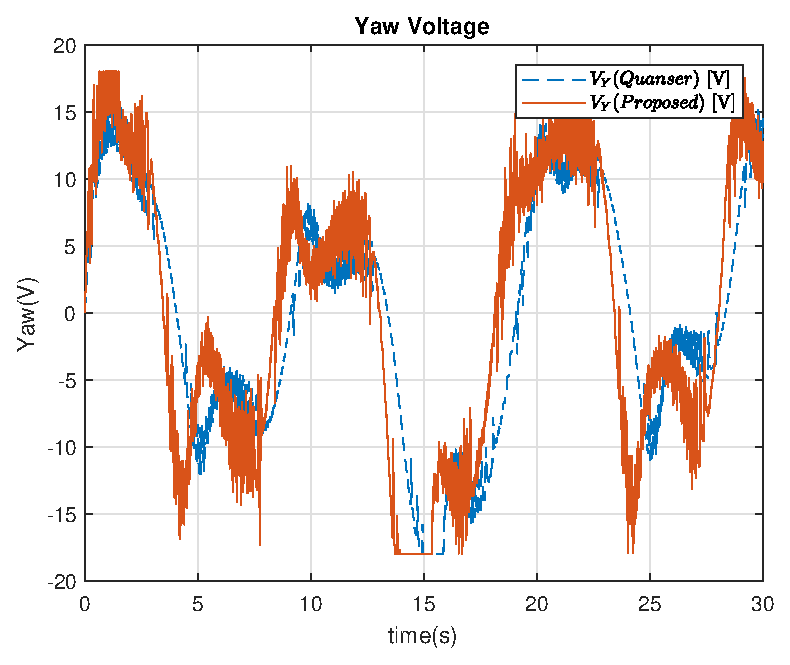
\includegraphics[width=.46\textwidth,keepaspectratio=true]{figs/matlab/LQR_PIvLQR_P_USB/sine/YawVoltage_LQR_RMSE.eps}
    \label{fig:YawVoltage_LQR_RMSE_Sine}
    }
    \subfigure[][]{
    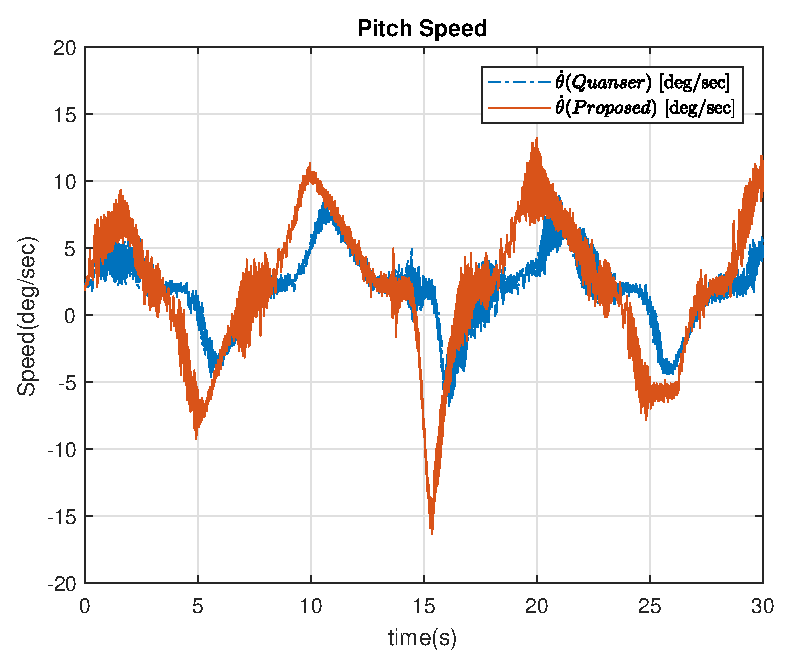
\includegraphics[width=.46\textwidth,keepaspectratio=true]{figs/matlab/LQR_PIvLQR_P_USB/sine/PitchSpeed_LQR_RMSE.eps}
    \label{fig:PitchSpeed_LQR_RMSE_Sine}
    }
    \subfigure[][]{
    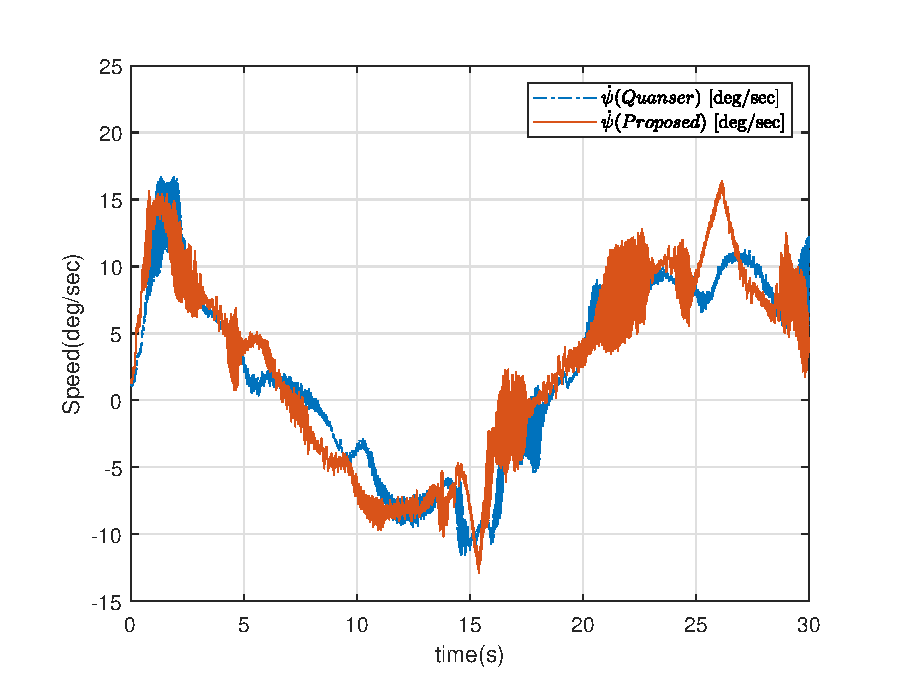
\includegraphics[width=.46\textwidth,keepaspectratio=true]{figs/matlab/LQR_PIvLQR_P_USB/sine/YawSpeed_LQR_RMSE.eps}
    \label{fig:PitchSpeed_LQR_RMSE_Sine}
    }
    \caption{USB implementation for proportional controller and proportional-integral controller calculated by LQR with a sinusoidal input.}
\end{figure}
%----------------------------------------------------------------------
\subsection{LQG (PI Controller)}
%----------------------------------------------------------------------
\todo[inline]{Insert LQG PI Block Diagram}
\todo[inline]{Insert LQG PI Results}
%----------------------------------------------------------------------
\subsection{ADP}
%----------------------------------------------------------------------
\todo[inline]{Insert ADP P Block Diagram}
\todo[inline]{Insert ADP P Results}

%----------------------------------------------------------------------
\subsection{Conclusions}
%----------------------------------------------------------------------
Note: constant used pitch 10 degrees, yaw 45 degrees\\
Note: square used pitch XXXX degrees with period of XXXX, yaw XXXX degrees with period of XXXX\\
Note: sine used pitch XXXX degrees with period of XXXX, yaw XXXX degrees with period of XXXX\\
\begin{table}[h!]
    \centering
    \begin{tabular}{l|l|l|l|l|l|l}
        \toprule
        \textbf{} & \textbf{LQR(P)} & \textbf{LQR(PI)} &
        \textbf{ADP(P)} \\
        \toprule
        RMSE Pitch Step & 2.6454 & ? & 1.3067 \\
        RMSE Yaw Step & 5.7991 & ? & 6.1991 \\
        RMSE Pitch Square & ? & ? & ? \\
        RMSE Yaw Square & ? & ? & ? \\
        RMSE Pitch Sine & ? & ? & ? \\
        RMSE Yaw Sine & ? & ? & ? \\
        \bottomrule
    \end{tabular}
    \caption{Error Comparison for USB Algorithms}
    \label{tab:USB_RMSE}
\end{table}
Based on the results XXXX preformed better for USB.
%----------------------------------------------------------------------

%======================================================================
\section{Raspberry Pi}

%----------------------------------------------------------------------
\subsection{LQR (P Controller)}
%----------------------------------------------------------------------

%----------------------------------------------------------------------
\subsection{ADP}
%----------------------------------------------------------------------

%----------------------------------------------------------------------
\subsection{Conclusions}
%----------------------------------------------------------------------
Note: constant used pitch XXXX degrees, yaw XXXX degrees\\
Note: square used pitch XXXX degrees with period of XXXX, yaw XXXX degrees with period of XXXX\\
Note: sine used pitch XXXX degrees with period of XXXX, yaw XXXX degrees with period of XXXX\\
\begin{table}[h!]
    \centering
    \begin{tabular}{l|l|l|l|l|l|l}
        \toprule
        \textbf{} & \textbf{LQR(P)} & \textbf{ADP(P)} \\
        \toprule
        RMSE Pitch Step & ? & ?  \\
        RMSE Yaw Step & ? & ? \\
        RMSE Pitch Square & ? & ? \\
        RMSE Yaw Square & ? & ? \\
        RMSE Pitch Sine & ? & ? \\
        RMSE Yaw Sine & ? & ? \\
        \bottomrule
    \end{tabular}
    \caption{Error Comparison for USB Algorithms}
    \label{tab:USB_RMSE}
\end{table}
Based on the results XXXX preformed better for Raspberry Pi.
%----------------------------------------------------------------------

%======================================================================
\section{Mobile Device}

%----------------------------------------------------------------------
\subsection{LQR (P Controller)}
%----------------------------------------------------------------------
\begin{figure}
    \centering
    \subfigure[][]{
    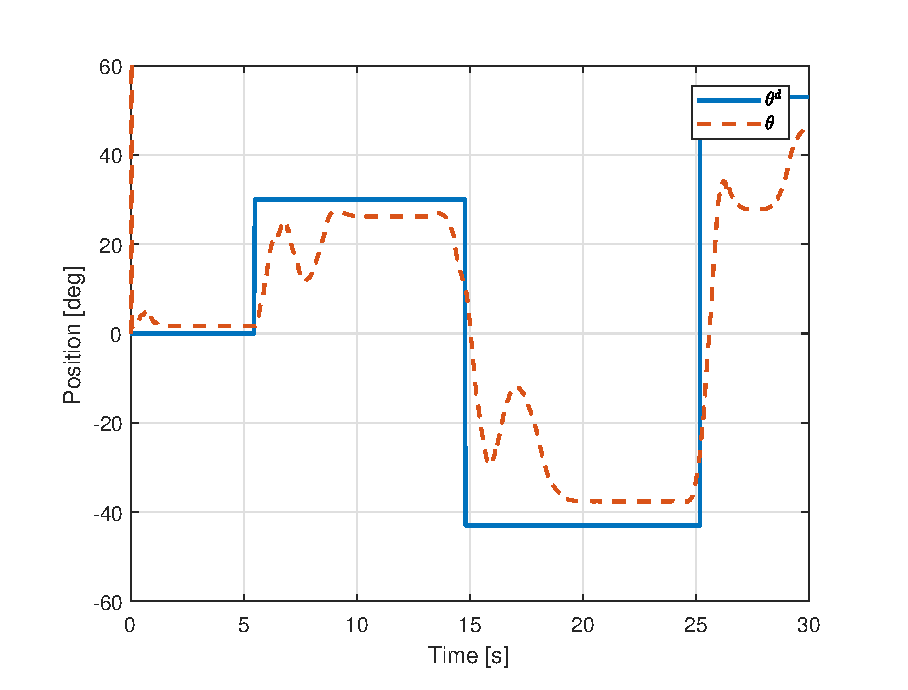
\includegraphics[width=.46\textwidth,keepaspectratio=true]{figs/matlab/LQR/P_Android/LQR_Pitchpos.eps}
    \label{fig:AndroidLQRPitchpos}
    }
    \subfigure[][]{
    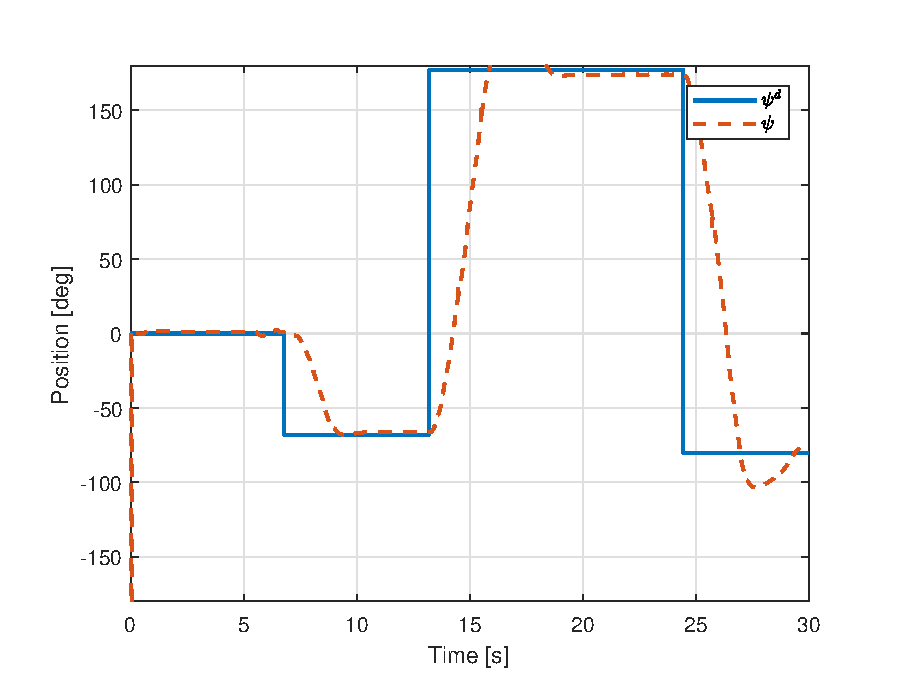
\includegraphics[width=.46\textwidth,keepaspectratio=true]{figs/matlab/LQR/P_Android/LQR_Yawpos.eps}
    \label{fig:AndroidLQRYawpos}
    }
    \subfigure[][]{
    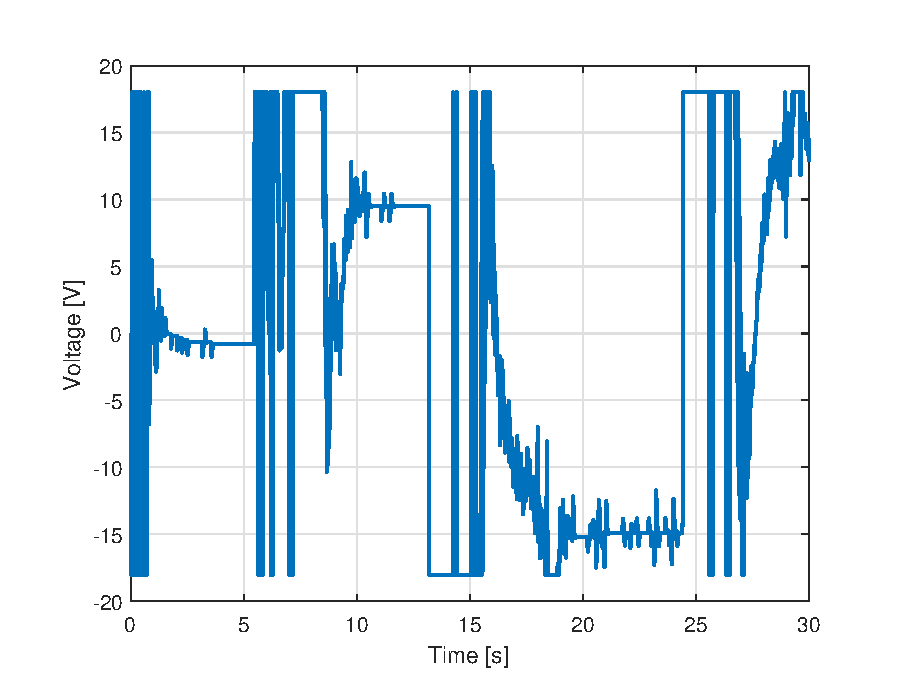
\includegraphics[width=.46\textwidth,keepaspectratio=true]{figs/matlab/LQR/P_Android/LQR_PitchVolt.eps}
    \label{fig:AndroidLQRPitchVolt}
    }
    \subfigure[][]{
    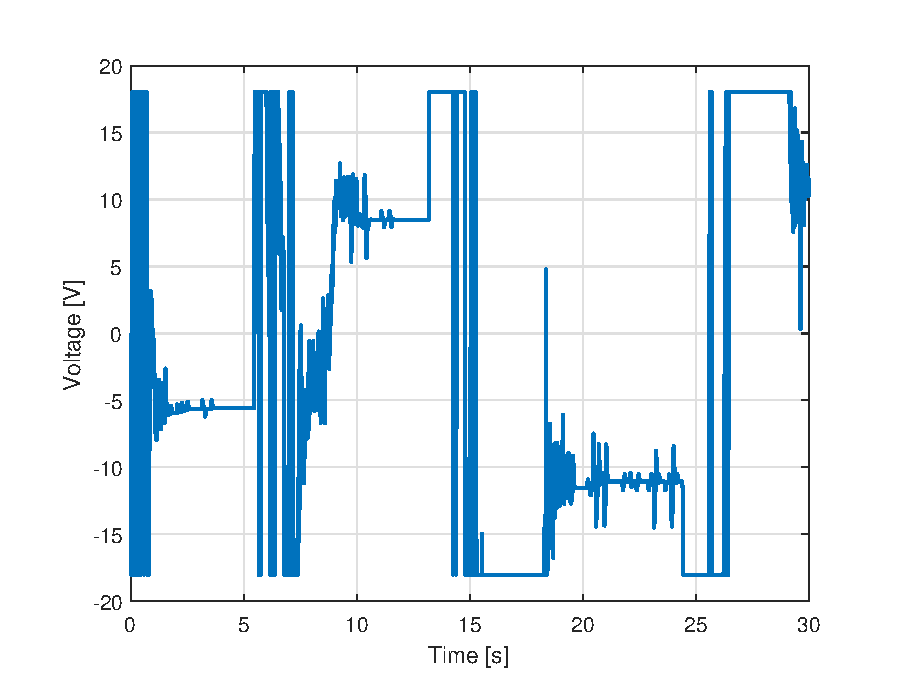
\includegraphics[width=.46\textwidth,keepaspectratio=true]{figs/matlab/LQR/P_Android/LQR_YawVolt.eps}
    \label{fig:AndroidLQRYawVolt}
    }
    \caption{LQR Android Results}
    \label{fig:AndroidLQR}
\end{figure}


%----------------------------------------------------------------------
\subsection{ADP}
%----------------------------------------------------------------------

\begin{figure}
    \centering
    \subfigure[][]{
    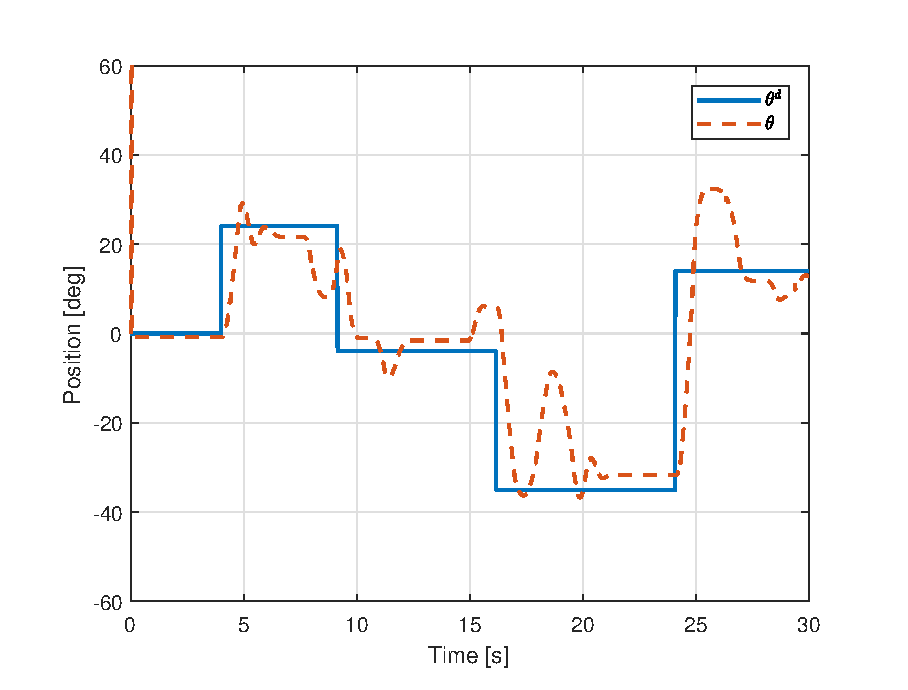
\includegraphics[width=.46\textwidth,keepaspectratio=true]{figs/matlab/ADP/Android/ADP_Pitch_Wireless.eps}
    \label{fig:AndroidADPPitchpos}
    }
    \subfigure[][]{
    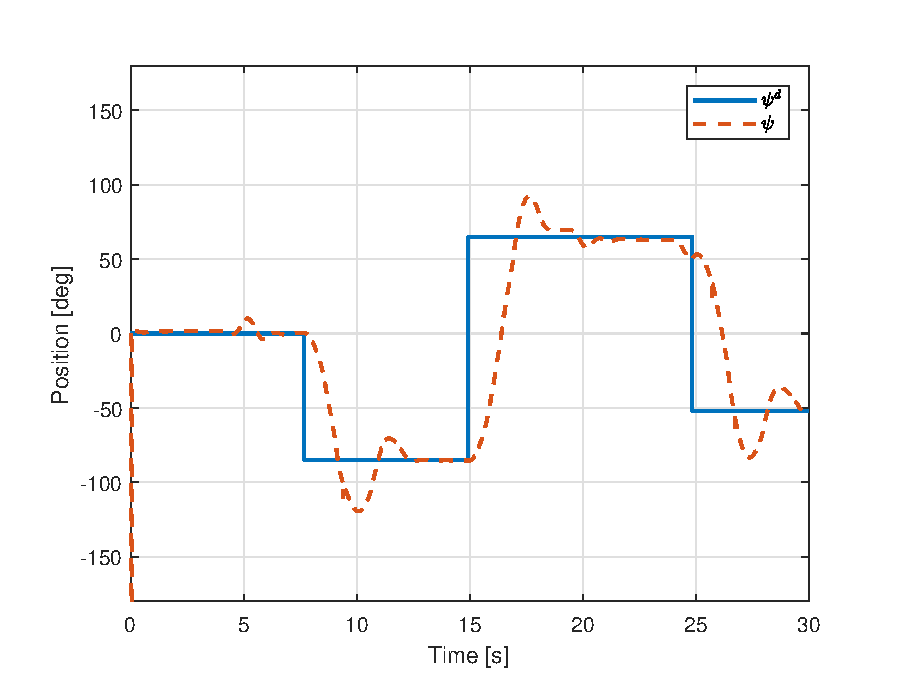
\includegraphics[width=.46\textwidth,keepaspectratio=true]{figs/matlab/ADP/Android/ADP_Yaw_Wireless.eps}
    \label{fig:AndroidADPYawpos}
    }
    \subfigure[][]{
    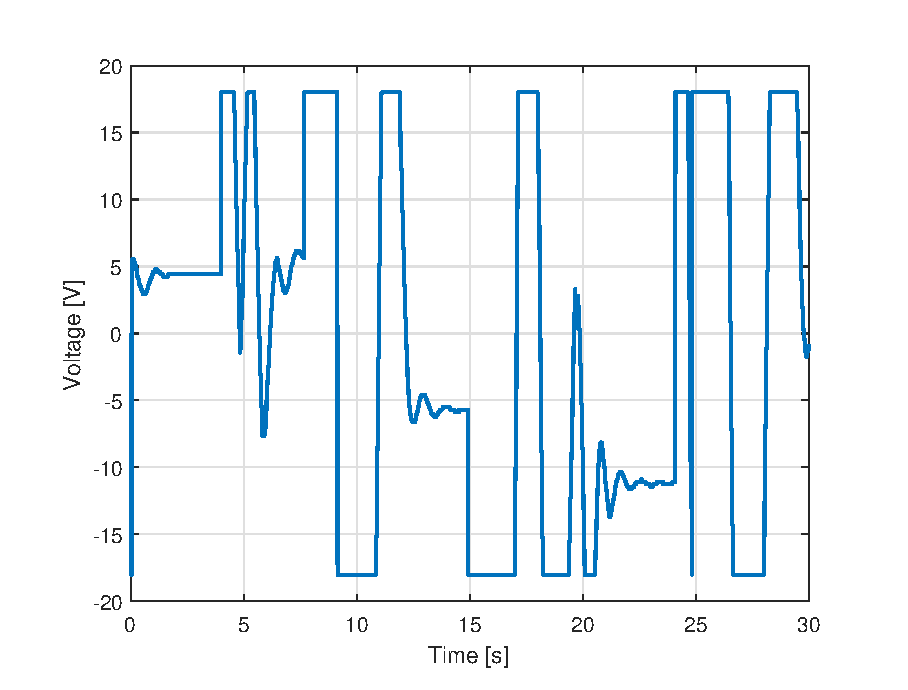
\includegraphics[width=.46\textwidth,keepaspectratio=true]{figs/matlab/ADP/Android/ADP_Pitch_Volt_Wireless.eps}
    \label{fig:AndroidADPPitchVolt}
    }
    \subfigure[][]{
    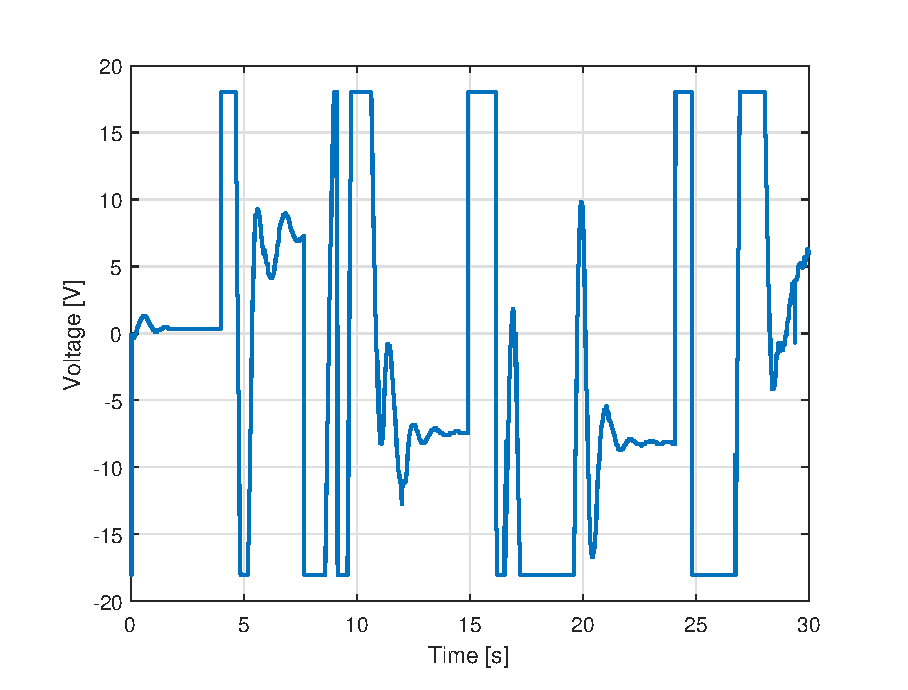
\includegraphics[width=.46\textwidth,keepaspectratio=true]{figs/matlab/ADP/Android/ADP_Yaw_Volt_Wireless.eps}
    \label{fig:AndroidADPYawVolt}
    }
    \caption{ADP Android Results}
    \label{fig:AndroidADP}
\end{figure}

%----------------------------------------------------------------------
\subsection{Conclusions}
%----------------------------------------------------------------------
Note: constant used pitch XXXX degrees, yaw XXXX degrees\\
Note: square used pitch XXXX degrees with period of XXXX, yaw XXXX degrees with period of XXXX\\
Note: sine used pitch XXXX degrees with period of XXXX, yaw XXXX degrees with period of XXXX\\
\begin{table}[h!]
    \centering
    \begin{tabular}{l|l|l|l|l|l|l}
        \toprule
        \textbf{} & \textbf{LQR(P)} & \textbf{ADP(P)} \\
        \toprule
        RMSE Pitch Step & ? & ?  \\
        RMSE Yaw Step & ? & ? \\
        RMSE Pitch Square & ? & ? \\
        RMSE Yaw Square & ? & ? \\
        RMSE Pitch Sine & ? & ? \\
        RMSE Yaw Sine & ? & ? \\
        \bottomrule
    \end{tabular}
    \caption{Error Comparison for USB Algorithms}
    \label{tab:USB_RMSE}
\end{table}
Based on the results XXXX preformed better for Android.

%----------------------------------------------------------------------


%%% Local Variables:
%%% mode: latex
%%% TeX-master: "../finalReport"
%%% End:
